\newpage
\section{Architecture of the system}
\label{sec:arch}
The block diagram of the system can be seen in Figure \ref{fig:arch}. The system starts calculating a initial path plan for the robot based on the initial state of the workspace. Then, periodically, the stereo camera provides two images, in which features of the ball are detected and used to triangulate the location of the ball in the real world. This triangulation is done by the epipolar lines method. This 3D coordinates are forwarded to the Kalman filter, which keeps track of the object more accurately. Once the 3D coordintate prediction is obtained, it is used for updating the environment of the robot and the collision map, in seek of potential collisions all along the path that was initially calculated.

All this information is sent to the planner of the robot, which based on it, determines if the robot can still stick to the initial plan to reach the goal or, it is necessary to replan the root to avoid obstacles that are now on the way.
\begin{figure}[H]
    \centering
    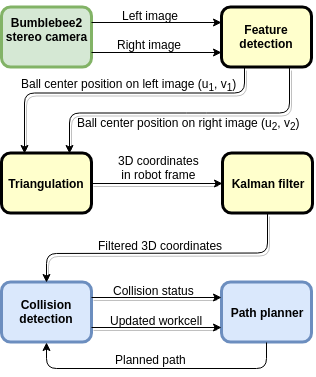
\includegraphics[width=0.7\textwidth]{Images/arch.png}
    \caption{Data flow}
    \label{fig:arch}
\end{figure}

This main structure has to be accommodated to the software used. To see the whole design of the system using ROS, go to section \ref{sec:ros}.